\section{\DualChain{} Architecture}
\label{s:dual}
Our \DualChain{} runs two distinct consensus protocols in parallel. 
Specifically, it requires the replicas in set $\Replicas{}$ to commit each client transaction
through a \BFT{} consensus protocol (commitment phase), following which the miners in set $\Miners{}$ run our \PoC{} 
consensus (settlement protocol). As all the \BFT{} protocols follow the consensus dictated by 
\pbft~\cite{pbftj}, we use \pbft{} as the representative protocol 
for the ensuing discussions.
%
{\em To summarize:} each client sends its request to the replicas running the \pbft{} protocol. 
Once these replicas commit this request, they forward it to the miners. 
These miners collaboratively run the \PoC{} consensus protocol, post 
which they add a block to the ledger. Next, we discuss each of these steps 
in detail.

\begin{figure}[t]
   \centering
   \begin{tikzpicture}[yscale=0.5,xscale=0.75]
       \draw[thick,draw=black!75] (1.75,   0) edge ++(10.5, 0)
                                  (1.75,   1) edge ++(10.5, 0)
                                  (1.75,   2) edge ++(10.5, 0)
                                  (1.75,   3) edge[blue!50!black!90] ++(10.5, 0)
                                  (1.75,   4) edge[green!50!black!90] ++(10.5, 0);

       \draw[thin,draw=black!75] (2, 0) edge ++(0, 4)
                                 (4,   0) edge ++(0, 4)
                                 (6, 0) edge ++(0, 4)
                                 (8,   0) edge ++(0, 4)
                                 (10,   0) edge ++(0, 4);

       \node[left] at (1.8, 0) {\scriptsize $\Replica_3$};
       \node[left] at (1.8, 1) {\scriptsize $\Replica_2$};
       \node[left] at (1.8, 2) {\scriptsize $\Replica_1$};
       \node[left] at (1.8, 3) {\scriptsize $\Primary{}$};
       \node[left] at (1.8, 4) {\scriptsize $\Client$};

       \path[->] (2, 4) edge [red!50](4, 3)
       
                 (4, 3) edge (6, 2)
                        edge (6, 1)
                        edge (6, 0)                        
                       
                 (6, 0) edge (8, 1)
                        edge (8, 2)
                        edge (8, 3)      
                
                 (6, 1) edge (8, 0)
                        edge (8, 2)
                        edge (8, 3)
                       
                 (6, 2) edge (8, 0)
                        edge (8, 1)
                        edge (8, 3)

                 (8, 0) edge (10, 1)
                        edge (10, 2)
                        edge (10, 3)
                       
                 (8, 1) edge (10, 0)
                        edge (10, 2)
                        edge (10, 3)
                       
                 (8, 2) edge (10, 0)
                        edge (10, 1)
                        edge (10, 3)
                       
                 (8, 3) edge (10, 0)
                        edge (10, 1)
                        edge (10, 2)
                 (10, 0) edge (12, 4)
                 (10, 1) edge (12, 4)
                 (10, 2) edge (12, 4)
                 (10, 3) edge (12, 4);
      
       \node[dot,colA] at (10, 0) {};
       \node[dot,colA] at (10, 1) {};
       \node[dot,colA] at (10, 2) {};
       \node[dot,colA] at (10, 3) {};
      
       \path (10, 3) edge[thick,colA] (10, -1.3);
       %\node[label,below right,align=left] at (10, 0) {\scriptsize \MName{Inform}};

       \node[label,below,yshift=3pt] at (3, 5) {\scriptsize \MName{$\Transaction$}};
       \node[label,below,yshift=3pt] at (5, 0) {\scriptsize \MName{PrePrepare}};
       \node[label,below,yshift=3pt] at (7, 0) {\scriptsize \MName{Prepare}};
       \node[label,below,yshift=3pt] at (9, 0) {\scriptsize \MName{Commit}};
       \node[label,below,yshift=3pt] at (11, 0) {\scriptsize \MName{Inform}};
   \end{tikzpicture}
   \caption{A schematic representation of the normal-case of the \pbft{} 
   protocol with $\n{\Replicas{}} = 4$ and $\f{\Replicas} = 1$. 
	%The primary $\Primary$ proposes a transaction $\Transaction{}$ submitted by client $\Client$ to all replicas via a $\MName{PrePrepare}$ message. Next, each replica broadcasts a $\MName{Prepare}$ message for $\T$. Upon a replica $\Replica$ receives $\NonFaulty_{pbft}$ for $\T$ from distinct replicas, $\Replica$ broadcasts a $\MName{Commit}$ message. Upon a replica $\Replica$ receives $\T$ from distinct replicas, execute $\T$ and inform $\Client$ the outcome.
	}
   \label{fig:pbft}
\end{figure}


\subsection{Client Request and Transaction Ordering}
\pbft{} follows the primary-backup model where one replica is designated as the 
{\em primary} while other replicas act as backups. Each consensus is led by the 
primary replica of the current {\em view}. In the case the primary is malicious, 
{\em view-change} takes place to replace the primary. We use Figure~\ref{fig:pbft} 
to illustrate the three phases of \pbft{}.


{\em Client Request.}
A client $\Client{}$ that wants to process a transaction $\Transaction{}$ in 
our \DualChain{} architecture creates a request $\SignMessage{\Transaction}{\Client{}}$ 
and sends it to the replica designated as the primary of the view $v$. The 
client $\Client{}$ uses \DS{} to sign this message and 
adds a monotonically increasing timestamp to this message.

{\em Pre-prepare.} 
When the primary $\Primary{}$ replica receives a well-formed client request 
$m := \SignMessage{\Transaction}{\Client{}}$, it assigns $m$ a sequence number 
$k$ and creates and sends a $\MName{Preprepare}$ message to all the replicas.
This $\MName{Preprepare}$ message also includes a digest $\Hash{m}$ of $m$, 
which is used in future communication to save space. During this phase, it is 
sufficient for the primary to sign the messages using \MAC{}.
%
When a replica $\Replica{} \in \Replicas{}$ receives a well-formed 
$\MName{Preprepare}$ message from the primary $\Primary{}$ of view $v$, it agrees 
to support the order $k$ for $m$ if it has not agreed to order another request 
at sequence number $k$. The replica $\Replica$ shows its support by broadcasting 
a $\MName{Prepare}$ message.

{\em Prepare.}
When a node $\Replica{}$ receives identical $\MName{Prepare}$ messages from 
$2\f{\Replicas{}}+1$ distinct replicas (can include its own message to reach the 
count), it marks the request $m$ as {\em prepared} and broadcasts a $\MName{Commit}$ 
message. In \DualChain, we require each replica $\Replica{}$ to use $\MName{DS}$ 
to sign the $\MName{Commit}$ message.

{\em Commit.}
When $\Replica{}$ receives identical $\MName{Commit}$ messages from 
$2\f{\Replicas{}}+1$ replicas, it marks $m$ as {\em committed}. If $\Replica{}$ 
has executed all requests with sequence number less than $k$, it executes $m$ and 
sends a $\MName{Response}$ message to the client, which includes the result of 
execution $r$. The client $\Client$ marks $\SignMessage{\Transaction}{\Client{}}$ 
as processed when it receives identical $\MName{Response}$ messages from at least 
$\f{\Replicas{}}+1$ replicas.

{\bf \em Chain Communication.} 
Post consensus on $m$, each replica $\Replica$ creates a certificate $\Certificate$, 
which includes: 
(i) the client request $m$,
(ii) $\MName{Commit}$ messages for $m$ from $2\f{\Replicas{}}+1$ replicas, and
(iii) the result $r$.
Next, the replicas may follow the {\em cluster-sending} protocol~\cite{byz-cluster-sending} 
or delayed replication protocol~\cite{delayedrepl} to communicate with the miners 
in set $\Miners$.\footnote{We can model chain communication as either push- or pull-based 
model using existing peer-to-peer communication primitives.} The cluster-sending 
protocol guarantees the delivery of at least one message between the two clusters, 
given that less than one-third of members of each cluster are malicious. To do so, 
each member from the sending cluster sends a message to a distinct member in the 
receiving member. In our case, we need the certificate $\Certificate$ to be sent to 
at least $2\f{\Miners}+1$ miners: replica $\Replica{1}$ sends $\Certificate$ to miner 
$\Miner_{1}$; replica $\Replica{2}$ sends $\Certificate$ to miner $\Miner_{2}$, and 
so on.


\begin{figure}[t]
   \centering
    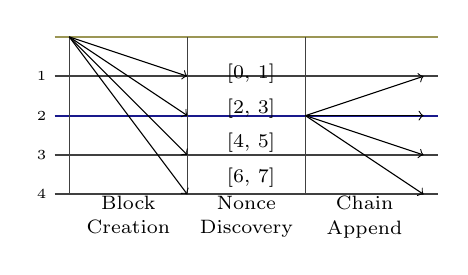
\begin{tikzpicture}[yscale=0.5,xscale=0.75]
           \draw[thick,draw=black!75] (1.75,   0) edge ++(6.5, 0)
                                   (1.75,   1) edge ++(6.5, 0)
                                   (1.75,   2) edge [blue!50!black!90] ++(6.5, 0)
                                   (1.75,   3) edge ++(6.5, 0)
                                   (1.75,   4) edge [yellow!50!black!90]++(6.5, 0);

           \node[label,below,yshift=3pt] at (3, 0) {\scriptsize \MName{Block}};
           \node[label,below,yshift=-6pt] at (3, 0) {\scriptsize \MName{Creation}};
           \node[label,below,yshift=3pt] at (5, 0) {\scriptsize \MName{Nonce}};
           \node[label,below,yshift=-6pt] at (5, 0) {\scriptsize \MName{Discovery}};
           \node[label,below,yshift=3pt] at (7, 0) {\scriptsize \MName{Chain}};
           \node[label,below,yshift=-6pt] at (7, 0) {\scriptsize \MName{Append}};
            
           \draw[thin,draw=black!75]   (2, 0) edge ++(0, 4)
                                       (4, 0) edge ++(0, 4)
                                       (6, 0) edge ++(0, 4);

           \node at (5, 1.8) {
                  \renewcommand{\arraystretch}{1.05}
           \begin{tabular}{c}
                  {\scriptsize[0, 1]}  \\
                  {\scriptsize[2, 3]}  \\
                  {\scriptsize[4, 5]}  \\
                  {\scriptsize[6, 7]}  \\
           \end{tabular}
           };

       \node[left] at (1.8, 0) {\scriptsize $\Miner_4$};
       \node[left] at (1.8, 1) {\scriptsize $\Miner_3$};
       \node[left] at (1.8, 2) {\scriptsize $\Miner_2$};
       \node[left] at (1.8, 3) {\scriptsize $\Miner_1$};
       \node[left] at (1.8, 4) {\scriptsize $\PBFT{}$};
       
       \path[->] (2, 4) 
                            edge (4, 3)                      
                            edge (4, 2)     
                            edge (4, 1)
                            edge (4, 0);
       \path[->] (6, 2) 
                            edge (8, 3)                      
                            edge (8, 2)
                            edge (8, 1)
                            edge (8, 0);

    \end{tikzpicture}
    	\caption{A schematic representation of the \PoC{} protocol with 
    	$\Miners{} = \{\Miner_1, \Miner_2, \Miner_3, \Miner_4\}$. 
    	The total solution space $\Slice{}$ is $[0,7]$ and is divided into four 
    	slices $([0,1], [2,3], [4,5], [6,7])$. Miners receive transactions from 
    	the \pbft{} replicas. Post creating a block, each Miner 
    	$\Miner_{i}$, $i \in [1,4]$ tries to discover the nonce in its slice 
    	$\Slice{i}$. Assume the valid nonce is $2$, then once $\Miner_2$ discovers 
    	the nonce, it broadcasts the same to other miners.
	}
	\label{fig:poc}
\end{figure}

When a miner $\Miner \in \Miners$ receives a certificate $\Certificate$ from 
a replica $\Replica \in \Replicas$, it broadcasts this certificate to all the 
other miners. As at least $2\f{\Miners}+1$ miners receive certificates, there 
is a guarantee that at least one honest miner will broadcast the certificate.
As a result, each miner will have access to the certificate $\Certificate$, and 
it can proceed with the \PoC{} computation.


\subsection{Collaborative Mining}
Post \pbft{} consensus, our \DualChain{} system runs the \PoC{} protocol on the 
agreed transaction to securely bind it to the ledger.
\PoC{} requires all the miners to {\em collaborate} and work together to compute 
the required hash. To do so, \PoC{} divides the \PoW{} hash computation into 
$\n{\Miners}$ disjoint subproblems and requires each miner to work on a distinct 
predetermined subproblem.

Let, $\Slice{}$ represent the solution space; all the random numbers that a miner 
has to try to find a valid nonce. Without the loss of generality, let us divide 
$\Slice{}$ into $\n{\Miners}$ equal slices, 
$\{ \Slice{1}, \Slice{2}, \cdots \Slice{\n{\Miners}} \}$, such that%

\begin{equation}
\Slice{1} \cap \Slice{2} \cap \cdots \cap \Slice{\n{\Miners}} = \varnothing 
\end{equation}%

\begin{equation}
\Slice{1} \cup \Slice{2} \cup \cdots \cup \Slice{\n{\Miners}} = \Slice{} 
\end{equation}

Our \PoC{} protocol assigns slice $\Slice{1}$ to miner $\Miner_{1}$, $\Slice{2}$ 
to $\Miner_{2}$, and $\Slice{i}$ to $\Miner_{i}$, $i \in [1,\n{\Miners}]$. The key 
assumption is that if a miner takes time $\tau$ to find a valid nonce on the solution 
space $\Slice{}$, then if all the miners are honest and follow the \PoC{} protocol, 
the time required to find the nonce should be of the order 
$\BigO{\dfrac{\tau}{\n{\Miners{}}}}$.

Further, \PoC{} protocol ensures that each honest miner gets rewarded for their 
efforts; rewards are distributed among miners. If $\Diamond$ is the reward for a 
miner to find a valid nonce in \PoW{} protocol, then in our \PoC{} protocol, each 
$i^{th}$ miner $\Miner_{i}$ receives a reward $\Diamond_i$ proportional to the size 
of its slice $\Slice{i}$.%

\begin{equation} 
    \Diamond_i = \frac{\abs{\Slice{i}}}{\abs{\Slice{}}} * \Diamond
\end{equation}

In the rest of this paper, for simplicity, we assume that all the slices have the same size.

\subsubsection{\PoC{} Protocol}
Our \PoC{} protocol works in rounds, and within each round each miner tries to find 
if a valid nonce exists in its slice of the block. In the rest of this section, we 
assume that the solution space $\Slice{}$ can be deterministically divided into 
$\n{\Miners{}}$ disjoint equal slices by each miner. For example, in Figure~\ref{fig:poc}, 
the solution space $\Slice{} = [0,7]$ is divided into $\n{\Miners{}} = 4$ slices; the 
slices are: $\Slice{1} = [0,1]$, $\Slice{2} = [2,3]$, $\Slice{3} = [4,5]$, and $\Slice{4} = [6,7]$.
Designing optimal slice distribution schemes is an interesting research avenue, which 
we consider outside the scope of this work.
%It contains two steps: obtain client transactions from $\PBFT{}$ network and mining the new block. We define the transactions in $\block_i$ mined in round i as $\TXNBlock_i$ and all $\TXNBlock_i$ are the same.

{\em Certificate Dissemination.} 
The \PoC{} protocol starts when a miner $\Miner{}$ receives a certificate $\Certificate$ 
from a replica. The miner $\Miner{}$ checks if $\Certificate$ is well-formed and 
$\Certificate$ includes signatures from $2\f{\Replicas{}}+1$ replicas; a proof that 
these replicas agreed to sequence this batch of transactions at a sequence number $k$.
If this is the case, $\Miner{}$ broadcasts this certificate to other miners.
Note: although while explaining \pbft{} we considered consensus on a single transaction, 
it can be trivially extended to a batch of transactions. This batching optimization is 
employed by all the existing \BFT{} protocols to increase their 
throughputs~\cite{pbftj,poe,rcc}.

{\em Block Creation.}
When a miner $\Miner$ has the nonce for the block ordered at sequence number $k-1$, 
it initiates the creation of a block at sequence $k$. It does so by generating a Merkle root 
of all the transactions in $k^{th}$ batch and a new block header. As each miner 
$\Miner{}$ knows there are a total of $\n{\Miners}$ miners, it creates $\n{\Miners}$ 
slices and assigns itself the $i^{th}$ slice $\Slice{i}$ in round $0$, where 
$i = \ID{\Miner{}}$.

{\em Nonce Discovery.}
We assume that each miner $\Miner{}$ knows the characteristics of the expected hash 
(the number of leading zeroes). The miner uses this information to go over all the 
possible nonces in its slice range to find a valid nonce. Once a miner $\Miner$ 
computes the correct hash, it has access to a valid nonce. The miner $\Miner$ uses 
this information to complete the block header and forwards the block to all the miners.

{\em Chain Append.}
When a miner receives a block from another miner, it first validates the nonce. If 
the nonce is valid, the miner appends this block to its local blockchain and assumes 
the \PoC{} protocol for the corresponding batch as complete.
% 
Notice that if all the miners are well-behaving, then our \PoC{} protocol requires 
only one round to find the valid nonce as the nonce is present in one of the slices.
Post discovering the nonce, each miner starts working on the next block to be added to 
the chain.

%\begin{figure}[t!]\label{ex:poc_no_solution}
%   \centering
%       \centering
%    \begin{tikzpicture}[yscale=0.5,xscale=0.75]
%           \draw[thick,draw=black!75] (0.75,   0) edge ++(14.5, 0)
%                                   (0.75,   1) edge ++(14.5, 0)
%                                   (0.75,   2) edge ++(14.5, 0)
%                                   (0.75,   3) edge ++(14.5, 0)
%                                   (0.75,   4) edge [yellow!50!black!90]++(14.5, 0);
%
%           \node[label,below,yshift=3pt] at (2, 0) {\scriptsize \MName{Block [$\block{1}$]}};
%           \node[label,below,yshift=3pt] at (4, 0) {\scriptsize \MName{Nonce}};
%           \node[label,below,yshift=-6pt] at (4, 0) {\scriptsize \MName{Discovery}};
%           \node[label,below,yshift=-15pt] at (4, 0) {\scriptsize \MName{(Timeout)}};
%           \node[label,below,yshift=3pt] at (6, 0) {\scriptsize \MName{Slice}};
%           \node[label,below,yshift=-6pt] at (6, 0) {\scriptsize \MName{Shift}};
%           \node[label,below,yshift=3pt] at (8, 0) {\scriptsize \MName{Nonce}};
%           \node[label,below,yshift=-6pt] at (8, 0) {\scriptsize \MName{Discovery}};
%           \node[label,below,yshift=-15pt] at (8, 0) {\scriptsize \MName{(Timeout)}};
%           \node[label,below,yshift=3pt] at (10, 0) {\scriptsize \MName{Block}};
%           \node[label,below,yshift=-6pt] at (10, 0) {\scriptsize \MName{[$\block{1}$, $\block{2}$]}};
%           \node[label,below,yshift=3pt] at (12, 0) {\scriptsize \MName{Nonce}};
%           \node[label,below,yshift=-6pt] at (12, 0) {\scriptsize \MName{Discovery}};
%           \node[label,below,yshift=3pt] at (14, 0) {\scriptsize \MName{Chain}};
%           \node[label,below,yshift=-6pt] at (14, 0) {\scriptsize \MName{Update}};
%            
%           \draw[thin,draw=black!75]   (1, 0) edge ++(0, 4)
%                                       (3, 0) edge ++(0, 4)
%                                       (5, 0) edge ++(0, 4)
%                                       (7, 0) edge ++(0, 4)
%                                       (9, 0) edge ++(0, 4)
%                                       (11, 0) edge ++(0, 4)
%                                       (13, 0) edge ++(0, 4.2);
%
%       \node[left] at (0.8, 0) {\scriptsize $\Miner_4$};
%       \node[left] at (0.8, 1) {\scriptsize $\Miner_3$};
%       \node[left] at (0.8, 2) {\scriptsize $\Miner_2$};
%       \node[left] at (0.8, 3) {\scriptsize $\Miner_1$};
%       \node[left] at (0.8, 4) {\scriptsize $\PBFT{}$};
%
%       \node at (4, 1.8) {
%                  \renewcommand{\arraystretch}{1.05}
%           \begin{tabular}{c}
%                  {\scriptsize \MName[0, 1]}  \\
%                  {\scriptsize \MName[2, 3]}  \\
%                  {\scriptsize \MName[4, 5]}  \\
%                  {\scriptsize \MName[6, 7]}  \\
%           \end{tabular}
%           };
%
%       \path[->] (1, 4) 
%                            edge (3, 3)                      
%                            edge (3, 2)     
%                            edge (3, 1)
%                            edge (3, 0);
%       \path[->] (5, 3) 
%                            edge (7, 3)                      
%                            edge (7, 2)     
%                            edge (7, 1)
%                            edge (7, 0);
%       \path[->] (5, 2) 
%                            edge (7, 3)                      
%                            edge (7, 2)     
%                            edge (7, 1)
%                            edge (7, 0);
%       \path[->] (5, 1) 
%                            edge (7, 3)                      
%                            edge (7, 2)     
%                            edge (7, 1)
%                            edge (7, 0);
%       \path[->] (5, 0) 
%                            edge (7, 3)                      
%                            edge (7, 2)     
%                            edge (7, 1)
%                            edge (7, 0);
%       \node at (8, 1.8) {
%                  \renewcommand{\arraystretch}{1.05}
%           \begin{tabular}{c}
%                  {\scriptsize \MName[2, 3]}  \\
%                  {\scriptsize \MName[4, 5]}  \\
%                  {\scriptsize \MName[6, 7]}  \\
%                  {\scriptsize \MName[0, 1]}  \\
%           \end{tabular}
%       };
%       \path[->] (9, 4) 
%                            edge (11, 3)                      
%                            edge (11, 2)     
%                            edge (11, 1)
%                            edge (11, 0);
%       \node at (12, 1.8) {
%                  \renewcommand{\arraystretch}{1.05}
%           \begin{tabular}{c}
%                  {\scriptsize \MName[0, 1]}  \\
%                  {\scriptsize \MName[2, 3]}  \\
%                  {\scriptsize \MName[4, 5]}  \\
%                  {\scriptsize \MName[6, 7]}  \\
%           \end{tabular}
%           };
%
%       \path[->] (13, 1) 
%                            edge (15, 3)                      
%                            edge (15, 2)     
%                            edge (15, 1)
%                            edge (15, 0);
%
%    \end{tikzpicture}
%    	\caption{An example that no valid nonce can be found for the new block. If the {\em timer} $\delta$ fires because no valid new block arrives,
%           a Slice Shifting will be triggered by sending a shift message <SHIFT, h, $\ShiftRound{i}$> to other miners. If a miner $\Miner{j}$ receives
%           $2\f{\Replicas}+1$ same shift messages from distinct miners, it starts its $\ShiftRound{i+1}$ by assigning its $\Slice{j}$ to $\Slice{j+1}$
%           and start to find the valid nonce in the new $\Slice{j}$. If no valid block has been found after $\f{\Miners{}}$ rounds, we can determine 
%           that there is no solution for this new block. The transactions $\Transaction{}$ in this block will be merged into the next block and skip the
%           current one. We assume nonce 3 is the valid value for the second block that contains $\block{1} and \block{2}$ in this example.
%           }
%\end{figure}\label{fig:poc_no_solution}

\begin{figure}
   \centering
    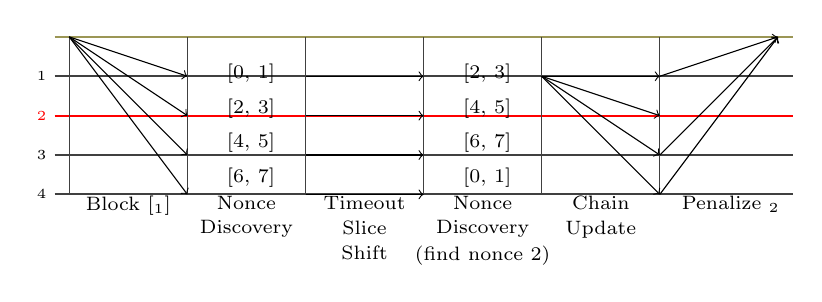
\begin{tikzpicture}[yscale=0.5,xscale=0.75]
           \draw[thick,draw=black!75] (0.75,   0) edge ++(12.5, 0)
                                   (0.75,   1) edge ++(12.5, 0)
                                   (0.75,   2) edge [red] ++(12.5, 0)
                                   (0.75,   3) edge ++(12.5, 0)
                                   (0.75,   4) edge [yellow!50!black!90]++(12.5, 0);

           \node[label,below,yshift=3pt] at (2, 0) {\scriptsize \MName{Block [$\block_{1}$]}};
           \node[label,below,yshift=3pt] at (4, 0) {\scriptsize \MName{Nonce}};
           \node[label,below,yshift=-6pt] at (4, 0) {\scriptsize \MName{Discovery}};
           \node[label,below,yshift=3pt] at (6, 0) {\scriptsize \MName{Timeout}};
           \node[label,below,yshift=-6pt] at (6, 0) {\scriptsize \MName{Slice}};
           \node[label,below,yshift=-15pt] at (6, 0) {\scriptsize \MName{Shift}};
           \node[label,below,yshift=3pt] at (8, 0) {\scriptsize \MName{Nonce}};
           \node[label,below,yshift=-6pt] at (8, 0) {\scriptsize \MName{Discovery}};
           \node[label,below,yshift=-15pt] at (8, 0) {\scriptsize \MName{(find nonce 2)}};
           \node[label,below,yshift=3pt] at (10, 0) {\scriptsize \MName{Chain}};
           \node[label,below,yshift=-6pt] at (10, 0) {\scriptsize \MName{Update}};
           \node[label,below,yshift=3pt] at (12.2, 0) {\scriptsize \MName{Penalize $\Miner_{2}$}};
            
           \draw[thin,draw=black!75]   (1, 0) edge ++(0, 4)
                                       (3, 0) edge ++(0, 4)
                                       (5, 0) edge ++(0, 4)
                                       (7, 0) edge ++(0, 4)
                                       (9, 0) edge ++(0, 4)
                                       (11, 0) edge ++(0, 4);
       \node[left] at (0.8, 0) {\scriptsize $\Miner_4$};
       \node[left] at (0.8, 1) {\scriptsize $\Miner_3$};
       \node[left,red] at (0.8, 2) {\scriptsize $\Miner_2$};
       \node[left] at (0.8, 3) {\scriptsize $\Miner_1$};
       \node[left] at (0.8, 4) {\scriptsize $\PBFT{}$};

       \node at (4, 1.8) {
                  \renewcommand{\arraystretch}{1.05}
           \begin{tabular}{c}
                  {\scriptsize \MName[0, 1]}  \\
                  {\scriptsize \MName[2, 3]}  \\
                  {\scriptsize \MName[4, 5]}  \\
                  {\scriptsize \MName[6, 7]}  \\
           \end{tabular}
           };

       \path[->] (1, 4) 
                            edge (3, 3)                      
                            edge (3, 2)     
                            edge (3, 1)
                            edge (3, 0);
       \path[->] (5, 3) 
                            edge (7, 3);
                            %edge (7, 2)     
                            %edge (7, 1)
                            %edge (7, 0);
       \path[->] (5, 2) 
                            %edge (7, 3)                      
                            edge (7, 2);     
                            %edge (7, 1)
                            %edge (7, 0);
       \path[->] (5, 1) 
                            %edge (7, 3)                      
                            %edge (7, 2)     
                            edge (7, 1);
                            %edge (7, 0);
       \path[->] (5, 0) 
                            %edge (7, 3)                      
                            %edge (7, 2)     
                            %edge (7, 1)
                            edge (7, 0);
       \node at (8, 1.8) {
                  \renewcommand{\arraystretch}{1.05}
           \begin{tabular}{c}
                  {\scriptsize \MName[2, 3]}  \\
                  {\scriptsize \MName[4, 5]}  \\
                  {\scriptsize \MName[6, 7]}  \\
                  {\scriptsize \MName[0, 1]}  \\
           \end{tabular}
       };
       \path[->] (9, 3) 
                            edge (11, 3)                      
                            edge (11, 2)     
                            edge (11, 1)
                            edge (11, 0);
       \path[->] (11, 3) 
                            edge (13, 4);
       \path[->] (11, 1) 
                            edge (13, 4);
       \path[->] (11, 0) 
                            edge (13, 4);

    \end{tikzpicture}
      \caption{An illustration of the slice shifting procedure. Here, we assume 
      $2$ is the valid nonce of the block, and the miner $\Miner_2$ is malicious. 
      Hence, $\Miner_2$ does not broadcast the block to other miners, which 
      triggers slice shifting procedure. Post slice shifting, $\Miner_1$ discovers 
      the nonce and broadcasts to other miners.
      }
	\label{fig:poc_malicious}
\end{figure}


\subsubsection{Slice Shifting Protocol}
In our \DualChain{} system, each miner receives certificates from the \pbft{} 
replicas. These certificates include client transactions that have been 
ordered by at least $2\f{\Replicas}+1$ replicas. Our \DualChain{} architecture 
uses the \PoC{} protocol to add these transactions to the ledger in the order 
defined by \pbft{} replicas. As a result, a malicious miner has limited attack 
opportunities; if a malicious miner finds a valid nonce in its slice, it can 
avoid forwarding this information to the honest miners. If such is the case, 
despite searching over its slice, each honest miner would not find any possible 
solution and would not be able to make progress.

To resolve this attack, our \PoC{} protocol requires each miner to set a 
{\em timer} $\delta$. Each miner $\Miner{}$ starts a timer $\delta$ when it 
receives a certificate from the \pbft{} replicas. $\Miner{}$ stops $\delta$ 
if it discovers the valid nonce or it receives a valid block from another miner.
If $\Miner{}$'s timer $\delta$ expires, and it does not have access to the valid 
nonce, it initiates the {\em slice shifting} protocol. Once the slice shifting 
is endorsed by the majority of miners, then each miner searches for the nonce 
in the next slice. Specifically, if prior to slice shifting a miner $\Miner{}$ 
was working on the $i^{th}$ slice $\Slice{i}$, post slice shifting $\Miner{}$ will 
work on $((i+1) \mod \n{\Miners{}})^{th}$ slice, $\Slice{(i+1)}$. As each miner 
already has access to all the slices, this switch does not require any 
additional communication.

The key intuition behind the slice shifting procedure is that even if a malicious 
miner decides to hide the nonce, post switch, it will be discovered by another miner.
However, it is possible that up to $\f{\Miners{}}$ consecutive miners may be malicious. 
As a result, the honest miners will discover the valid nonce after $\f{\Miners{}}$ shifts.%
\footnote{
The search space can be salted deterministically upon shifting to expand the search 
space and guard against rare cases in which the original problem may have no solution irrespective of minors' behavior.
}

%We impose all the solutions of $\PoW{}$ puzzles to be resolved in time T. (It is easy to restrict the solution time by modifying the difficulty, like Bitcoin estimate each block will be created average in 15 minutes and the longest mining time is no large than 2 hours from the median mining time of the previous 11 blocks[???]). 


\subsubsection{Reward and Penalty Economy}
Frequent slice shifting due to malicious miners will be detrimental to the 
performance of our \PoC{} protocol; it forces honest miners to do more work and 
wastes their resources. Moreover, why would any rational miner want to join the 
\PoC{} network and invest its computational resources? To make \PoC{} protocol 
fruitful, we incentivize all the honest miners for their efforts; all miners 
are assumed honest until proven guilty. 

First, like existing blockchain systems, such as Bitcoin and Ethereum, one of 
the aims of our \DualChain{} system is to establish a decentralized economy. 
To do so, like Bitcoin, in \PoC{}, when a miner discovers a nonce and broadcasts 
the valid block to other miners, we assume the creation of a {\em new token}. For 
brevity, we skip diving into the crypto-economics of the token generation and 
disbursement, and refer to the existing literature on the same~\cite{bitcoin,ether}. 
However, the key goal is that this token is equally divided among the honest 
miners. Further, like Bitcoin and Ethereum, we expect each client to pay some 
fees for getting its transaction processed by our \DualChain{} system. This 
fees is also equally divided among all the miners working on the current block.

To disburse transaction fees and tokens among the miners, there are two possible 
approaches: 
(i) Like Bitcoin, each miner includes $\n{\Miners{}}$ transactions that assigns an 
equal fraction of the reward to every other miner's public-key (account). These 
transactions can be deterministically created by each miner prior to mining and are 
included while creating the Merkle root. However, this will create unnecessary 
book-keeping, increasing the size of blocks.
(ii) We assume that the genesis block of the ledger records 
the information about the founding miners and their respective initial slices.
Further, miners can redistribute, resale, and divide their slices to other miners 
(similar to buying and selling of stocks), and any such transactions must be stored 
on the ledger before becoming effective. Assume that when a miner purchases a slice, 
sufficient tokens are reserved to enable penalization of misbehaving miners, 
which results in slashing their reserve funds similar to Proof-of-Stake 
designs~\cite{blockchain-book}. Given all this information, when a block is 
formed by the \PoC{} miners, we add the incentives to the accounts of
the respective miners; miners can validate if they received incentives or not. 

This rewarding process of \PoC{} is similar to strategies adopted by 
{\em mining pools} in systems like Bitcoin. Most importantly, in \PoC{}, the 
agreement on what to be included in the next block is strictly determined by \PBFT{} 
chain, not miners. This substantially simplifies the design of \PoC{} by making it 
deterministic, eliminating any lottery-based or leader-less consensus challenges 
that traditional \PoW{} must cope with. Furthermore, we present the novel idea of 
slice shifting for the cases when no miner in a round broadcasts a valid nonce. 
As slice shifting requires each miner to work on the next slice to find the nonce, 
it is expensive. We mitigate the need for slice shifting by heavily {\em penalizing} 
malicious miners. Specifically, we require each miner to count the number of 
{\em shifts} it took to find a valid nonce and to identify the miner who failed 
to find the valid nonce. Further, as the order of all initial slice assignments is known 
to all the miners, so each miner can trivially determine which miner was responsible 
for previous shifts. Notice that any misbehaving miner will be discovered and penalized 
as it diminishes the returns for other honest miners. 


%\begin{lemma}
%    If a non-faulty miner finds out the solution and broadcasts the new block in the ShiftRound $\ShiftRound{i}$, at least $2*\f{\Miners{}}+1$ miners will receive 
%    the new block in $\ShiftRound{i}$ if the following assumptions are ture [...].
%\end{lemma}


%We use pay-per-share(PPS)[???] as a reward stratery. Whenever a new block is created, every miner will receive the reward 
%according to their exploring solution space ($\Slice$). 
%


%Once a miner receives a new block in its shift round $\ShiftRound_i$, it believes that the solution owners on $[\ShiftRound_1 \cdots \ShiftRound_{i-1}$ are faulty 
%and should be punished, by sneding a new message <PENALIZE, Miners, height> via $\PBFT{}$ network where Miners are the faluty 
%minters who did not work on the solution in the previous shift round, heigh is the current block height. Once a replica in $\PBFT{}$ network
%receives $2*F^{\PoW{}}+1$ same penalty messages from different miners, send a <PENALIZE\_ACK,Miners,height> to the current primary.
%Once the current primary receives $2*F^{\PBFT{}}+1$ PENALIZE\_ACK messages from distinct replicas, submit the PENALIZE\_ACK message via a
%new transaction by $\PBFT{}$ consensus algorithm. This transaction will be executed by all the miners eventually thought $\PoC$ protocol.
%(Figure $\ref{fig:penalty_normal_case}$)
%
%If a replica in $\PBFT{}$ network sends out a PUSHNISH\_ACK to the primary but does not receive the commit message in some timeouts, it will re-send
%the messages. If the committed message still does not arrive after some retry, it will trigger a ViewChange to change the current primary 
%(Figure $\ref{fig:penalty_timeout}$). 
%
%\input{punishment_nc}
